
\chapter{Results}

This is an example paragraph. As you can see, the main text uses a font size of 12 pt and a line spacing of 1.5. Neither the paragraphs nor the first lines of paragraphs should be indented.

There is no stringent page limit. The size and the total number of your figures and tables will strongly influence your number of pages. It is recommended to stay within 30-50 pages. Do not try to fill as many pages as you can. Longer theses are not necessarily of higher quality and have more non-redundant content than shorter theses. Indeed, a master thesis of 15 pages is too short, and a master thesis of 100 pages is too long.

\section{Tables and graphics}

This is an example paragraph. As you can see, the main text uses a font size of 12 pt and a line spacing of 1.5. Neither the paragraphs nor the first lines of paragraphs should be indented.

There is no very strict page limit. Your number of pages will be strongly influenced by the size and total number of your figures and tables. It is recommended staying within 30-50 pages. Do not try to fill as many pages as you can. Longer theses are not necessarily of higher quality and of more non-redundant content than shorter theses. Certainly, a master thesis of 15 pages is too short, and a master thesis of 100 pages is too long.

\begin{figure}[!ht]
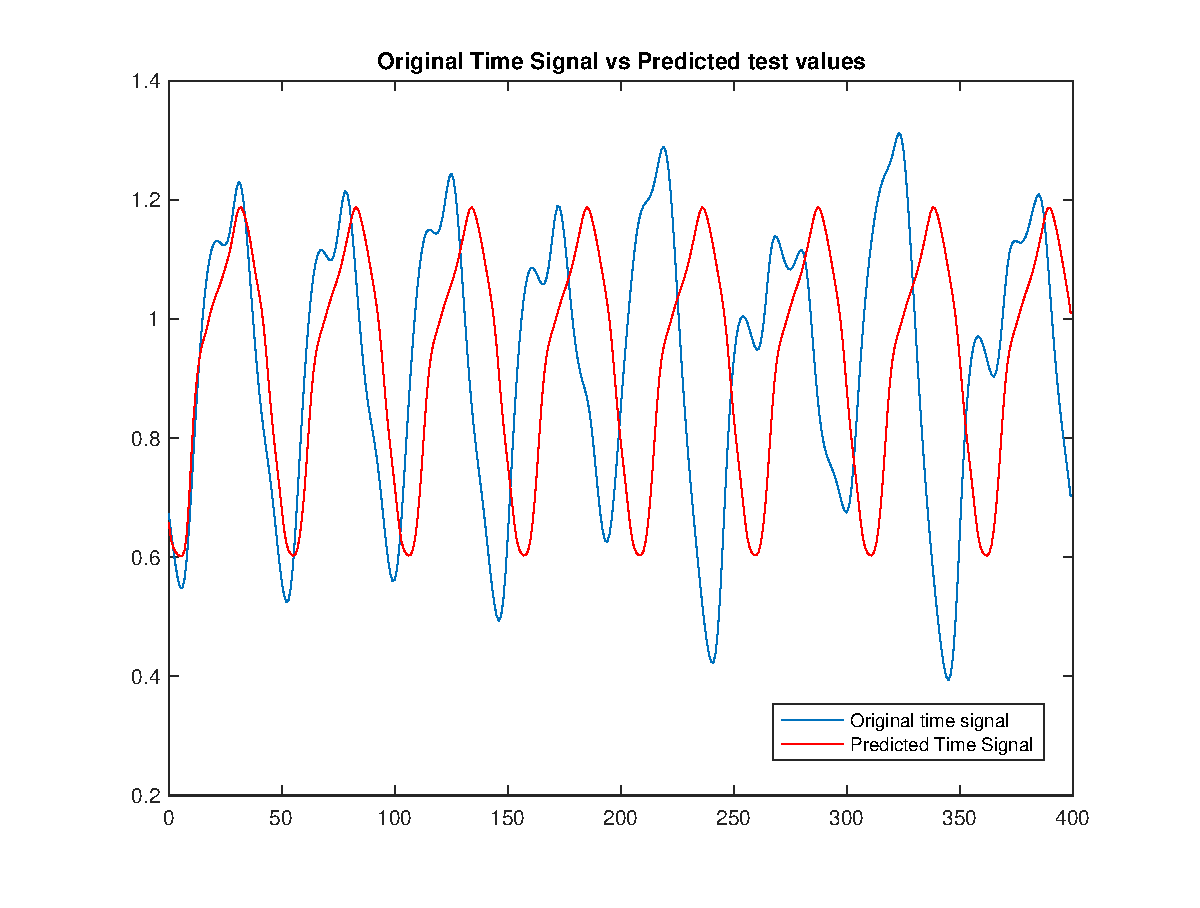
\includegraphics[clip,width=\columnwidth]{figures/PlotTimeSeriesResult}% 
\caption{This is an example of a figure and its caption.}
\label{fig:timeseries}
\end{figure}

\begin{table}[!ht]
\renewcommand{\arraystretch}{1.50}
\caption{This is an example of a table and its caption.}
\label{tablePCA}
\centering
\begin{tabular}{| c | c |}
\hline
\bfseries PCA & \bfseries Residual mean (in absolute values) \\
\hline\hline
Original PCA & 0.1267  \\
\hline
PCA on Centroid 1 & 0.1249\\
\hline
PCA on Centroid 2 & 0.1214  \\
\hline
\end{tabular}
\end{table}

\newpage


